\documentclass[border=3pt,tikz, convert]{standalone}
\usepackage{amsmath} % for aligned
\usepackage{listofitems} % for \readlist to create arrays
\usetikzlibrary{arrows.meta} % for arrow size
\usepackage[outline]{contour} % glow around text
\contourlength{1.4pt}

\usetikzlibrary{shapes.geometric}

% COLORS
\usepackage{xcolor}
\colorlet{myred}{red!80!black}
\colorlet{myblue}{blue!80!black}
\colorlet{mygreen}{green!60!black}
\colorlet{myorange}{orange!70!red!60!black}
\colorlet{mydarkred}{red!30!black}
\colorlet{mydarkblue}{blue!40!black}
\colorlet{mydarkgreen}{green!30!black}

% STYLES
\tikzset{
  >=latex, % for default LaTeX arrow head
  node/.style={thick,circle,minimum size=55,inner sep=0.5,outer sep=0.6},
  square/.style={thick, regular polygon,regular polygon sides=4, minimum size=45,inner sep=0.5,outer sep=0.6},
  node known/.style={node,black ,draw=black,fill=white},
  node unknown/.style={square,black,draw=black,fill=myblue!15},
  node convol/.style={node,orange!20!black,draw=myorange!30!black,fill=myorange!20},
  node out/.style={node,red!20!black,draw=myred!30!black,fill=myred!20},
  connect/.style={thick,mydarkblue}, %,line cap=round
  connect arrow/.style={-{Latex[length=4,width=3.5]},thick,mydarkblue,shorten <=0.5,shorten >=1},
  node 1/.style={node known}, % node styles, numbered for easy mapping with \nstyle
  node 2/.style={node known},
  node 3/.style={node out}
}

\begin{document}

% simple computational graph

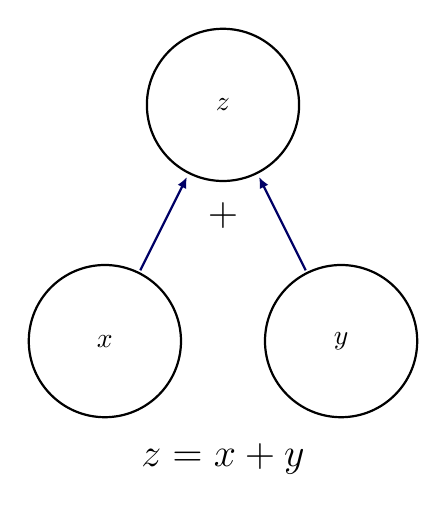
\begin{tikzpicture}
    \node[node known] (x) at (0,0) {$x$};
    \node[node known] (y) at (3,0) {$y$};
    \node[node known] (z) at (1.5,3) {$z$};
    \draw[connect arrow] (x) -- (z);
    \draw[connect arrow] (y) -- (z);
    \node (f) at (1.5,1.6) {\Large $+$};
    \node at (1.5, -1.5) {\Large $z = x + y$};
\end{tikzpicture}

% neural network (forward pass)

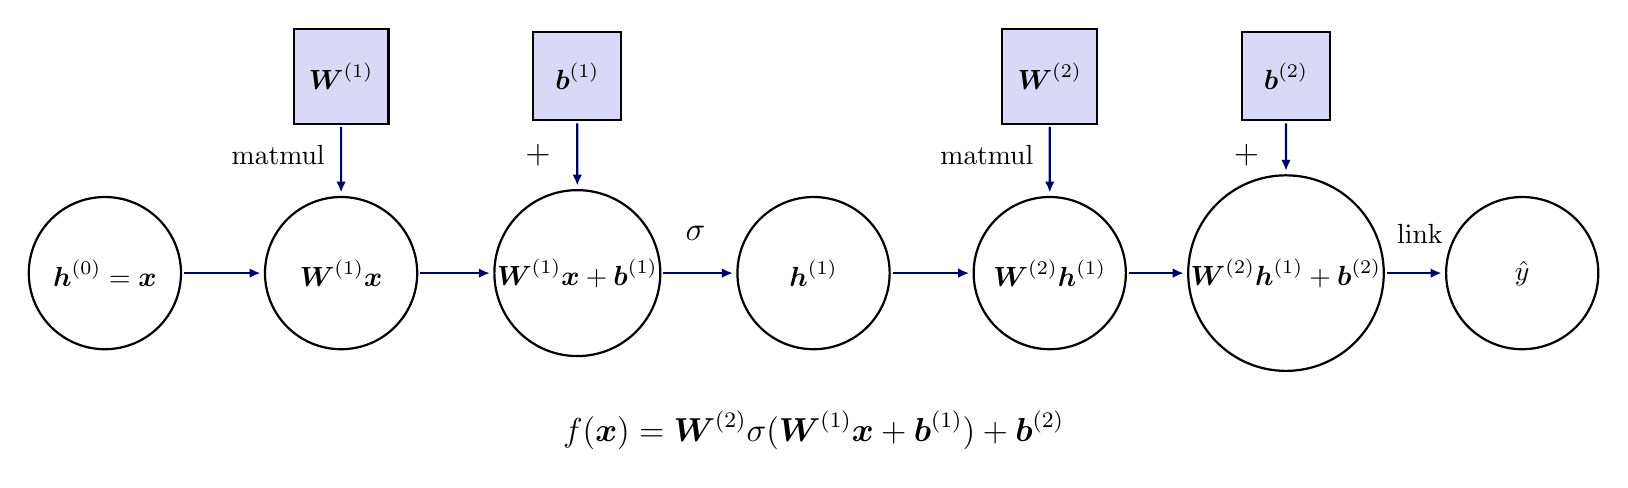
\begin{tikzpicture}
    \node[node known] (x) at (0,0) {$\boldsymbol{h}^{(0)} = \boldsymbol{x}$};
    \node[node unknown] (w1) at (3,2.5) {$\boldsymbol{W}^{(1)}$};
    \node[node known] (w1x) at (3,0) {$\boldsymbol{W}^{(1)}\boldsymbol{x}$};
    \node[node unknown] (b1) at (6,2.5) {$\boldsymbol{b}^{(1)}$};
    \node[node known] (w1xb) at (6,0) {$\boldsymbol{W}^{(1)}\boldsymbol{x} + \boldsymbol{b}^{(1)}$};
    \node[node known] (h1) at (9,0) {$\boldsymbol{h}^{(1)}$};
    \node[node known] (w2h) at (12,0) {$\boldsymbol{W}^{(2)}\boldsymbol{h}^{(1)}$};
    \node[node known] (w2hb) at (15,0) {$\boldsymbol{W}^{(2)}\boldsymbol{h}^{(1)} + \boldsymbol{b}^{(2)}$};
    \node[node unknown] (w2) at (12, 2.5) {$\boldsymbol{W}^{(2)}$};
    \node[node unknown] (b2) at (15, 2.5) {$\boldsymbol{b}^{(2)}$};
    \node[node known] (y_hat) at (18,0) {$\hat{y}$};
    
    \draw[connect arrow] (x) -- (w1x);
    \draw[connect arrow] (w1) -- (w1x) ;
    \node at (2.2, 1.5) {matmul};
    \draw[connect arrow] (b1) -- (w1xb) ;
    \node at (5.5, 1.5) {\large $+$};
    \draw[connect arrow] (w1x) -- (w1xb) ;
    \draw[connect arrow] (w1xb) -- (h1);
    \node at (7.5,0.5) {\large $\sigma$};
    \draw[connect arrow] (h1) -- (w2h);
    \draw[connect arrow] (w2) -- (w2h);
    \draw[connect arrow] (w2h) -- (w2hb);
    \node at (11.2, 1.5) {matmul};
    \draw[connect arrow] (b2) -- (w2hb);
    \node at (14.5, 1.5) {\large $+$};
    \draw[connect arrow] (w2hb) -- (y_hat);
    \node at (16.7,0.5) {link};

    \node at (9, -2) {\large $f(\boldsymbol{x}) = \boldsymbol{W}^{(2)}\sigma(\boldsymbol{W}^{(1)}\boldsymbol{x} + \boldsymbol{b}^{(1)}) + \boldsymbol{b}^{(2)}$};
    
\end{tikzpicture}

% neural network (backward pass) 

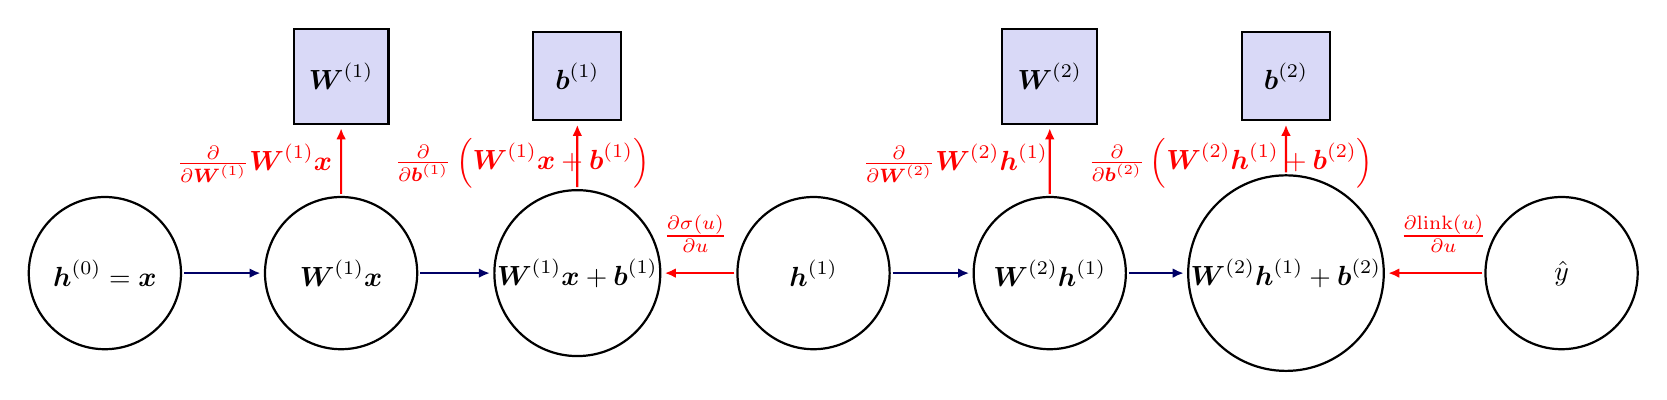
\begin{tikzpicture}
  \node[node known] (x) at (0,0) {$\boldsymbol{h}^{(0)} = \boldsymbol{x}$};
  \node[node unknown] (w1) at (3,2.5) {$\boldsymbol{W}^{(1)}$};
  \node[node known] (w1x) at (3,0) {$\boldsymbol{W}^{(1)}\boldsymbol{x}$};
  \node[node unknown] (b1) at (6,2.5) {$\boldsymbol{b}^{(1)}$};
  \node[node known] (w1xb) at (6,0) {$\boldsymbol{W}^{(1)}\boldsymbol{x} + \boldsymbol{b}^{(1)}$};
  \node[node known] (h1) at (9,0) {$\boldsymbol{h}^{(1)}$};
  \node[node known] (w2h) at (12,0) {$\boldsymbol{W}^{(2)}\boldsymbol{h}^{(1)}$};
  \node[node known] (w2hb) at (15,0) {$\boldsymbol{W}^{(2)}\boldsymbol{h}^{(1)} + \boldsymbol{b}^{(2)}$};
  \node[node unknown] (w2) at (12, 2.5) {$\boldsymbol{W}^{(2)}$};
  \node[node unknown] (b2) at (15, 2.5) {$\boldsymbol{b}^{(2)}$};
  \node[node known] (y_hat) at (18.5,0) {$\hat{y}$};
  
  \draw[connect arrow] (x) -- (w1x);
  \draw[connect arrow, red] (w1x) -- (w1) ;
  \node at (1.9, 1.4) {$\textcolor{red}{\frac{\partial}{\partial \boldsymbol{W}^{(1)}} \boldsymbol{W}^{(1)} \boldsymbol{x}}$};
  \draw[connect arrow, red] (w1xb) -- (b1) ;
  \node at (5.3, 1.4) {$\textcolor{red}{\frac{\partial}{\partial \boldsymbol{b}^{(1)}}\left(\boldsymbol{W}^{(1)} \boldsymbol{x} + \boldsymbol{b}^{(1)}\right)}$};
  \draw[connect arrow] (w1x) -- (w1xb) ;
  \draw[connect arrow, red] (h1) -- (w1xb);
  \node at (7.5,0.5) {$\textcolor{red}{\frac{\partial \sigma(u)}{\partial u}}$};
  \draw[connect arrow] (h1) -- (w2h);
  \draw[connect arrow, red] (w2h) -- (w2);
  \draw[connect arrow] (w2h) -- (w2hb);
  \node at (10.8, 1.4) {$\textcolor{red}{\frac{\partial}{\partial \boldsymbol{W}^{(2)}}\boldsymbol{W}^{(2)} \boldsymbol{h}^{(1)}}$};
  \draw[connect arrow, red] (w2hb) -- (b2);
  \node at (14.3, 1.4) {$\textcolor{red}{\frac{\partial}{\partial \boldsymbol{b}^{(2)}}\left(\boldsymbol{W}^{(2)} \boldsymbol{h}^{(1)} + \boldsymbol{b}^{(2)}\right)}$};
  \draw[connect arrow, red] (y_hat) -- (w2hb);
  \node at (17,0.5) {$\textcolor{red}{\frac{\partial \text{link}(u)}{\partial u}}$};
  
\end{tikzpicture}



\end{document}